Der Security Manager (SM) bzw. das Security Manager Protocol (SMP) ist dafür zuständig, eine sichere Verbindung zwischen zwei Geräten (Master und Slave) aufzubauen. Dies umfasst im Wesentlichen das Pairing, das zur Authentifizierung und Generierung eines Schlüssels dient, und die Verteilung von Schlüsseln. Entsprechend der Abb. \ref{fig: smp in bt} lässt sich der Security Manager bzw. das SMP in die BLE-Architektur einordnen.

\begin{figure}[H]
    \centering
    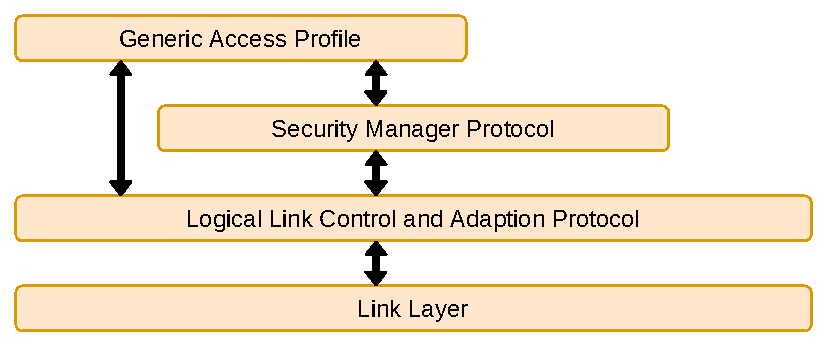
\includegraphics[width=0.8\textwidth]{graphics/smp_in_bt.pdf}
    \caption[Beziehungen des Security Managers zu anderen Host-Komponenten]{Beziehungen des Security Managers zu anderen Host-Komponenten; in Anlehnung an \cite{BtSpec4.0_fig_1958}}
    \label{fig: smp in bt}
\end{figure}
% QUELLE Spec 4.0 S. 1958

Um mit dem Link Layer zu interagieren, nutzt der SM einen L2CAP Channel mit einer festgelegten CID. Zudem kann er mit GAP direkt kommunizieren.
\\\\
Das Pairing lässt sich in drei Phasen aufteilen. Phase 1 und 2 dienen der Generierung eines Schlüssels, den beide Geräte zur Verschlüsselung und Authentifizierung im Link Layer nutzen. Dafür wird der Cipher Block Chaining - Message Authentication Code (CCM) Mode in Verbindung mit dem Advanced Encryption Standard (AES), genauer dem AES-128 Block Cipher, genutzt \cite{BtSpec4.0_2285}.
% QUELLE Spec. 4.0 S. 2285, 1 ENCRYPTION AND AUTHENTICATION OVERVIEW

\paragraph{Pairing: Phase 1} \mbox{} \vspace{0.2cm} \\
Die erste Phase ist der Pairing Feature Exchange, bei dem die beiden Geräte ihre für den Nutzer zugänglichen Ein- und Ausgabemöglichkeiten (IO Capabilities) austauschen. Die Tabellen \ref{tab: i caps geraet} und \ref{tab: o caps geraet} 
listen die entsprechenden Bezeichnungen dieser Möglichkeiten auf.
\\\\

\begin{table}[H]
    \begin{tabularx}{\textwidth}{|l|X|}
    \hline
    \textbf{Eingabemöglichkeit} & \textbf{Beschreibung} \\
    \hline
    Keine Eingabe & Gerät kann keine Eingaben entgegennehmen \\
    \hline
    Ja / Nein & Gerät kann zwei verschiedene Eingaben verarbeiten, die der Bedeutung Ja bzw. Nein zugewiesen werden können (bspw. zwei Tasten) \\
    \hline
    Tastatur & Eingabe der Ziffern 0 bis 9 möglich und die Möglichkeit Ja und Nein einzugeben \\
    \hline
    \end{tabularx}
    \caption[Eingabemöglichkeiten eines Gerätes]{Eingabemöglichkeiten eines Gerätes \cite{BtSpec4.0_1965}}
    \label{tab: i caps geraet}
\end{table}

\begin{table}[H]
    \begin{tabularx}{\textwidth}{|l|X|}
    \hline
    \textbf{Ausgabemöglichkeiten} & \textbf{Beschreibung} \\
    \hline
    Keine Ausgabe & Gerät kann dem Nutzer keine sechsstellige Dezimalzahl anzeigen bzw. kommunizieren \\
    \hline
    Numerische Ausgabe & Gerät kann dem Nutzer eine sechsstellige Dezimalzahl anzeigen bzw. kommunizieren \\
    \hline
    \end{tabularx}
    \caption[Ausgabemöglichkeiten eines Gerätes]{Ausgabemöglichkeiten eines Gerätes \cite{BtSpec4.0_1965_b}}
    \label{tab: o caps geraet}
\end{table}
% QUELLE für Tabellen: Spec 4.0 S. 1965 Table 2.1 und Table 2.2

Desweiteren tauschen die Geräte in der ersten Phase Informationen darüber aus, ob eine Authentifizierung zum Schutz vor einem Man-In-The-Middle-Angriff nötig ist (MITM Flag), und ob Daten für die Authentifizierung über die Pairing-Methode Out Of Band (OOB), d.h. mittels einer anderen Technologie (z.B. Near Field Communication), übertragen werden können (OOB Flag). Außerdem werden die minimalen und maximalen Größen für die Schlüssel ausgetauscht, die sich in 8 Bit großen Schritten zwischen 56 Bit (7 Byte) und 128 Bit (16 Byte) befinden. Dabei wird das Minimum beider maximaler Größen übernommen. Falls die beiden Spannen sich nicht überschneiden, wird das Pairing abgebrochen.

\paragraph{Pairing: Phase 2} \mbox{} \vspace{0.2cm} \\
Anhand der ausgetauschten Informationen aus der ersten Phase wird in der zweiten Phase entschieden, welche der folgenden Methoden zur Generierung des Short Term Key (STK) bzw. Long Term Key (LTK) zu verwenden ist:
\begin{itemize}
    \item{Numeric Comparison (für LE erst ab Bluetooth-Version 4.2)}
    \item{Just Works}
    \item{Out of Band (OOB)}
    \item{Passkey Entry}
\end{itemize}
Da das Pairing (speziell Phase 2) für LE in der Bluetooth-Version 4.0 funktionale Unterschiede zum Pairing für LE ab Version 4.2 aufweist, wird das Pairing für LE in Version 4.0 als \textbf{LE Legacy Pairing} und das Pairing für LE ab Version 4.2 als \textbf{LE Secure Connections Pairing} bezeichnet. Aus Sicht des Nutzers sind beide Verfahren jedoch gleich und jede Bluetooth-Version, die LE unterstützt, unterstützt das LE Legacy Pairing. Im Gegensatz zum LE Secure Connections Pairing bietet LE Legacy Pairing für die Methoden Just Works und Passkey Entry keinen Schutz vor passivem Abhören während des Pairings, da LE Secure Connections Elliptic Curve Diffie-Hellman (ECDH) für den Schlüsselaustausch nutzt und LE Legacy Pairing nicht. \cite{BtSpec4.2_248}
% QUELLE Spec 4.2 S. 248 5.4.1 Association Models
\\\\
Verfügen beide Geräte über OOB-Authentifizierungsdaten für das LE Legacy Pairing, wird unabhängig vom jeweiligen MITM-Flag die Methode OOB gewählt. In LE Secure Connections Pairing wird ebenso verfahren, nur dass hier nicht die OOB-Flags beider Geräte gesetzt sein müssen (aber können), da ein gesetztes OOB-Flag genügt. Sind die MITM-Flags beider Geräte nicht gesetzt, wird die Methode Just Works ausgeführt. Anderenfalls werden die Ein- und Ausgabemöglichkeiten der Geräte entsprechend \cite{BtSpec4.2_tab_2302-2303} in die Wahl der Methode einbezogen.
% Verweis TABELLE Spec 4.2 S. 2302 f., Table 2.8

\subparagraph{Pairing Methoden} \mbox{} \vspace{0.2cm} \\
Bei der \textbf{Numeric Comparison} wird dem Nutzer auf beiden Geräten jeweils eine zufällig generierte sechsstellige Dezimalzahl angezeigt. Diese muss der Nutzer vergleichen und im Falle der Übereinstimmung auf beiden Geräten bestätigen oder anderenfalls ablehnen. Somit kann der Nutzer unabhängig von der Namensgegebung der Geräte sicherstellen, die richtigen Geräte ausgewählt zu haben. Zudem bietet diese Methode Schutz vor MITM-Angriffen. Außenstehende, die Kenntnis über diese Zahl gewonnen haben, können laut \cite{BtSpec4.2_244-245} damit keinen Vorteil zur Entschlüsselung der zwischen den beiden Geräten ausgetauschten Daten erlangen, da die Zahl nicht als Eingabe zur Generierung eines Schlüssels verwendet wird.
% QUELLE VERWEIS Sepc 4.2 S. 244 f. 5.2.4.1 Numeric Comparison

\textbf{Just Works} basiert auf der Funktionsweise von Numeric Comparison mit dem Unterschied, dass hier dem Nutzer keine sechsstellige Dezimalzahl ausgegeben wird und er die Verbindung nur bestätigen muss. Dadurch bietet Just Works keinen Schutz vor MITM-Angriffen, aber einen Schutz gegen passives Abhören (außer für LE Legacy Pairing). \cite{BtSpec4.2_245}
% QUELLE Spec 4.2 S.245 5.2.4.2 Just Works

\textbf{Out of Band} ist die Nutzung einer anderen Technologie (z.B. Near Field Communication), um Geräte zu entdecken oder um kryptographische Informationen für den Pairing-Prozess auszutauschen. Dabei sollte die Technologie Schutz vor MITM-Angriffen bieten. \cite{BtSpec4.2_246}
% QUELLE Spec 4.2 S. 246 5.2.4.3 Out of Band

Die Methode \textbf{Passkey Entry} definiert, dass ein Gerät die zufällig generierte sechstellige Dezimalzahl ausgibt und der Nutzer sie auf dem anderen Gerät eingeben muss. Ein Schutz gegen MITM-Angriffe ist gegeben, da diese nur mit einer Wahrscheinlichtkeit von 0,0001\% für jede Durchführung der Methode möglich sind. Schutz gegen passives Abhören bietet Passkey Entry nur in LE Secure Connections Pairing und nicht in LE Legacy Pairing. \cite{BtSpec4.2_246-247} \cite{BtSpec4.2_2304}
% QUELLE Spec 4.2 S. 246 f. 5.2.4.4 Passkey Entry
% QUELLE Spec. 4.2 S. 2304 2.3.5.3 LE Legacy Pairing - Passkey Entry

\subparagraph{LE Legacy Pairing: Schlüssel und deren Generierung} \mbox{} \vspace{0.2cm} \\
Beim LE Legacy Pairing zweier Geräte generieren beide einen 128 Bit langen Temporary Key (TK), der bei der Authentifizierung genutzt wird, um den STK zu generieren und die Verbindung zu verschlüsseln. In Just Works wird der TK auf null gesetzt. Bei der Methode Passkey Entry ist der TK die besagte zufällig generierte sechstellige Dezimalzahl, die bereits mit 20 Bit dargestellt werden kann, weswegen die restlichen Bit des TK auf null gesetzt werden müssen. Dagegen kann bei OOB auf diese Einschränkung verzichtet werden, wodurch der TK tatsächlich eine Länge von 128 Bit aufweist.
\\\\
Das Gerät, welches das Pairing einleitet (Master), generiert eine zufällige 128 Bit lange Nummer \textit{Mrand} und ermittelt den gleichlangen Bestätigungswert \textit{Mconfirm} mit der Confirm Value Generation Function c1 \cite{BtSpec4.2_2288}. 
% QUELLE Spec. 4.2 S. 2288 2.2.3 Confirm value generation function c1 for LE Legacy Pairing
Zur Berechnung von \textit{Mconfirm} erhält die Funktion c1 folgende Eingabewerte entsprechend Gl. \ref{eq: mconfirm} \cite{BtSpec4.2_2305-2306}:
\begin{equation}
\begin{split}
    \text{Mconfirm} = \text{c1}(& \text{TK, Mrand,} \\
    & \text{Pairing Request Command, Pairing Response Command,} \\
    & \text{Adresstyp des Masters, Adresse des Masters,} \\
    & \text{Adresstyp des Slaves, Adresse des Slaves}) \\
\end{split}
    \label{eq: mconfirm}
\end{equation}
Ebenso führt das antwortende Gerät (Slave) diese Schritte durch, wobei \textit{Mrand} als \textit{Srand} bezeichnet wird und \textit{Mconfirm} als \textit{Sconfirm}. Die Eingabewerte der Funktion c1 zur Berechnung von \textit{Sconfirm} sind demnach analog zu denen von \textit{Mconfirm}. Danach findet gemäß Abb. \ref{fig: austausch vor stk generierung} folgender Austausch statt:

\begin{figure}[H]
    \centering
    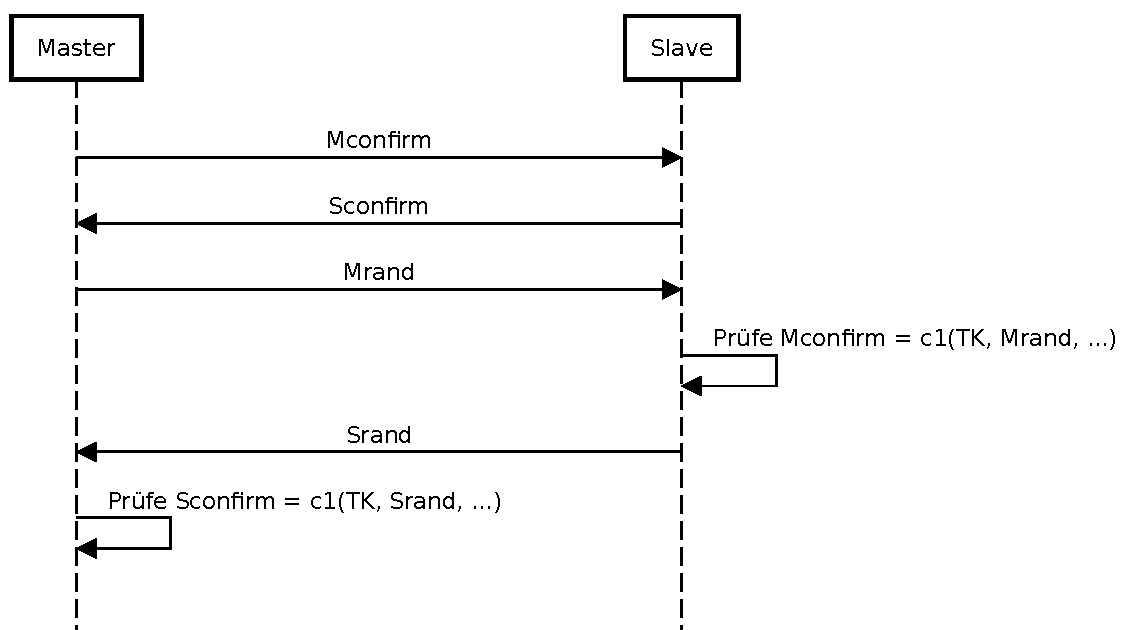
\includegraphics[width=0.9\textwidth]{graphics/austausch_vor_stk_generierung.pdf}
    \caption[Austausch von \textit{Mconfirm}, \textit{Sconfirm}, \textit{Mrand} und \textit{Srand} zwischen Master und Slave]{Austausch von \textit{Mconfirm}, \textit{Sconfirm}, \textit{Mrand} und \textit{Srand} zwischen Master und Slave \cite{BtSpec4.2_2305-2306}}
    \label{fig: austausch vor stk generierung}
\end{figure}

Master und Slave tauschen \textit{Mconfirm} und \textit{Sconfirm} aus. Danach überträgt der Master \textit{Mrand}, damit der Slave \textit{Mconfirm} entsprechend Gl. \ref{eq: mconfirm} berechnen und so den empfangenen \textit{Mconfirm} verifizieren kann. Nach einer erfolgreichen Prüfung von \textit{Mconfirm} überträgt der Slave \textit{Srand}, damit der Master \textit{Sconfirm} analog zu Gl. \ref{eq: mconfirm} berechnen und somit den empfangenen \textit{Sconfirm} verifizieren kann. Wenn einer der Bestätigungswerte (\textit{Mconfirm}, \textit{Sconfirm}) nicht erfolgreich verifiziert wird, wird die Verbindung sofort beendet.
\\\\
Anschließend wird der STK mit der Funktion s1 \cite{BtSpec4.2_2290} 
% QUELLE verweis auf Spec 4.2 S. 2290 2.2.4 Key generation function s1 for LE Legacy Pairing
entsprechend Gl \ref{eq: stk} \cite{BtSpec4.2_2305-2306} berechnet.

\begin{equation}
    \text{STK} = \text{s1}(\text{TK, Srand, Mrand})
    \label{eq: stk}
\end{equation}

Demnach kann bei der Methode Passkey Entry kein ausreichender Schutz gegen passives Abhören geboten werden, da der TK nur wenig mögliche Werte annehmen kann. Ist die vereinbarte Schlüsselgröße kleiner als 128 Bit, werden die überschüssigen Bit beginnend bei dem MSB auf null gesetzt. Der STK wird nun zur Verschlüsselung der Verbindung genutzt. \cite{BtSpec4.2_2305-2306}
% QUELLE Spec. 4.2 S. 2305 f. 2.3.5.5 LE Legacy Pairing Phase 2

\subparagraph{LE Secure Connections Pairing: Schlüssel und deren Generierung} \mbox{} \vspace{0.2cm} \\
Beim LE Secure Connections Pairing wird ein Long Term Key (LTK) erstellt. Zuvor generieren beide Geräte jeweils ein ECDH-Schlüsselpaar (PK - Public Key, SK - Private Key) und tauschen ihre Public Keys aus. Danach berechnet jedes Gerät den Diffie-Hellman-Schlüssel aus seinem Private Key und dem Public Key des Gegenübers. Durch den Diffie-Hellman-Schlüssel kennen beide Parteien ein gemeinsames Geheimnis, mit dem sie den weiteren Datenaustausch zur Authentifizierung verschlüsseln können. Die Authentifizierung ist notwendig, da der ECDH-Schlüsselaustausch zwar resistent gegen passives Abhören ist, jedoch nicht gegen MITM-Angriffe. \cite{BtSpec4.2_2307}
% QUELLE Spec. 4.2 S. 2307 2.3.5.6.1 Public Key Exchange

Diese Authentifizierung wird mit den Pairing Methoden Numeric Comparison, Just Works, OOB und Passkey Entry ermöglicht. Jedoch unterscheiden diese sich aus funktionaler Sicht (nicht aus Nutzersicht) vom LE Legacy Pairing durch komplexere Verfahren. Letztendlich lässt sich für die vier Pairing-Methoden Folgendes zusammenfassen: 
\begin{itemize}
    \item Numeric Comparison signalisiert dem Nutzer mit einer Wahrscheinlichkeit von 99,9999\% einen stattfindenden MITM-Angriff \cite{BtSpec4.2_2309}
% QUELLE Spec. 4.2 S. 2309, 2.3.5.6.2 Authentication Stage 1 – Just Works or Numeric Comparison
    \item Just Works bietet keinen Schutz vor einem MITM-Angriff \cite{BtSpec4.2_245} 
% QUELLE Spec. 4.2 S. 245, 5.2.4.2 Just Works
    \item Ein MITM-Angriff während des Passkey Entry gelingt nur mit einer Wahrscheinlichkeit von 0,0001\% \cite{BtSpec4.2_2311}
% QUELLE Spec. 4.2 S. 2311, 2.3.5.6.3 Authentication Stage 1 – Passkey Entry
    \item Anfälligkeit auf Angriffe bei der OOB-Methode ist von der verwendeten OOB-Technologie abhängig \cite{BtSpec4.2_2312-2313}
% QUELLE Spec. 4.2 S. 2312 f., 2.3.5.6.4 Authentication Stage 1 – Out of Band
\end{itemize}

Nach der Ausführung einer Pairing-Methode wird der LTK als Teilergebnis der Funktion f5 \cite{BtSpec4.2_2292-2293} 
% QUELLE Spec. 4.2 S. 2292 f., 2.2.7 LE Secure Connections Key Generation Function f5
mit den Eingabewerten Diffie-Hellman-Key, einer Nonce des Masters, einer Nonce des Slaves und der Adresse des Masters und Slaves ermittelt \cite{BtSpec4.2_2314}.
% QUELLE Spec. 4.2 S. 2314, 2.3.5.6.5 Authentication Stage 2 and Long Term Key Calculation

\paragraph{Pairing: Phase 3} \mbox{} \vspace{0.2cm} \\
Wurde der STK bzw. LTK generiert, wird er genutzt, um die Verbindung zu verschlüsseln. Nun können in der dritten Phase transportspezifische Schlüssel ausgetauscht werden. Z.B. wird der Identity Resolving Key (IRK) zur Generierung und Auflösung von zufälligen Adressen verwendet und der Connection Signature Resolving Key (CSRK) zur Signatur von Daten und Überprüfung von Signaturen.

% Für Numeric Comparison und Just Works wird entsprechend Abb. X fortgefahren.
% % TODO BILD VERWEIS

% \begin{figure}[hbt!]
%     \centering
%     \inlcudegraphics[width=0.5\linewidth]{graphics/LE_Secure_Connections_Pairing_Numeric_Comparison_Just_Works.svg}
%     \caption{}
% \end{figure}

% Der zu Beginn zufällig generierte Nonce (N\textunderscore a bzw. N\textunderscore b) mit einer Länge von 128 Bit wird für jeden Durchlauf neu erzeugt und schützt vor Replay-Angriffen. Für die Berechnung der Bestätigung C\textunderscore b wird die Einwegfunktion f4 [X] genutzt. 
% % TODO QUELLE Spec. 4.2 S. 2291 2.2.6 LE Secure Connections Confirm Value Generation Function f4
% Mittels der Funktion g2 [X] 
% % TODO QUELLE Spec 4.2 S. 2295 2.2.9 LE Secure Connections Numeric Comparison Value Generation Function g2
% werden die Dezimalzahlen D\textunderscore a und D\textunderscore b berechnet. Darauf werden diese dem Nutzer auf den Geräten ausgegeben und dieser muss deren Gleichheit bestätigen. Wird anstatt Numeric Comparison die Methode Just Works ausgeführt, dann werden D\textunderscore a und D\textunderscore b nicht berechnet und folglich nicht dem Nutzer gezeigt. Sollte ein Fehler auftreten wird das Protokoll abgebrochen und kann neu gestartet werden.

% Beim vorherigen ECDH-Schlüsselaustausch, kann ein MITM-Angriff angewandt werden. Eine einfache Variante, die keine Informationen der beiden angegriffenen Geräte zwischen diesen austauscht sondern mit diesen jeweils separat die Methode Numeric Comparison durchführt, endet darin, dass dem angegriffenem Nutzer mit einer Wahrscheinlichkeit von 0,999999 auf dessen Geräten zwei verschiedene Dezimalzahlen angezeigt werden. Eine andere Variante wäre aus Sicht des Angreifenden den Verkehr bestehend aus der Bestätigung C\textunderscore b, dem Nonce N\textunderscore a und N\textunderscore b nur weiterzuleiten. Jedoch wird der Master bei der Überprüfung der Bestätigung C\textunderscore b feststellen, dass diese nicht mit seinem Public Key PK\textunderscore a erstellt wurde, was zum Abbruch führt.\\\\
% % TODO QUELLE Spec. 4.2 S. 2308 f. 2.3.5.6.2 Authentication Stage 1 – Just Works or Numeric Comparison
% Passkey Entry
% OOB